\titleformat{\subsection}{\large\bfseries\CJKsection}{\thesubsection}{1em}{}

\chapter{\term{HIP} 工具 - 黃煒智}
\label{chap:HIP Tools}

正如我們之前所提,ROCm OS 提供的 HIP 支援大幅簡化了平行 GPU 程式的建立。然而,要達到最佳效能,更深入了解最適合的方法是必須的。有些人也許會透過反覆嘗試去調適出最佳效能。然而,效能分析工具透過提供系統化方法,能夠幫助所有人節省時間與精力,同時最大限度地減少混亂。除此之外,針對不同的 GPU 架構開發或移植應用程序是個挑戰,尤其是移植CUDA應用程式到新的架構。在本章節,我們將探討 ROCm 提供的工具用來分析及移植到不同的 GPU 架構。

ROCm提供程式設計者 \term{ROCmInfo},這命令列工具提供有關 ROCm 軟體堆疊和系統硬體配置的詳細資訊。開發者可以在最佳化效能時,快速且簡單的獲取系統設定的重要資訊。另外一個有用的工具是 ROCm System Management Interface (SMI,系統管理介面),可以幫助GPU程式設計者視覺化監控GPU的使用率、頻率、溫度等等的變數。根據操作系統的權限級別,程式設計者可以使用 ROCm SMI 去修改 GPU kernel和記憶體頻率(在設備允許的範圍內)。為了定位及調適kernel的錯誤,ROCm提供允許讓程式設計者逐步執行kernel原始碼的GNU除錯器(GDB) rocgdb。它可以檢查wavefront暫存器狀態。ROCm 也提供程式設計者 \term{rocProf},一個簡單使用的GPU硬體分析器,提供給應用程式開發者了解程式在GPU的行為是如何以及幫助辨識潛在的效能瓶頸。ROCm 提供將CUDA編寫的整個程式碼庫轉換到HIP的工具。有數種情況程式設計者或研究人員需要在AMD GPU上運行NVIDIA系統的CUDA程式,包含比較效能的差異。在HIP之前,只有涉及手動轉換從CUDA變成OpenCL的映射方法,一種繁瑣且容易出錯的路徑。章節 \chapref{chap:Third-Party Tools} 也提供各種第三方工具的指引,可以用來分析ROCm支援的GPU效能。

\section{\term{ROCmInfo}}

每當談到最大化效能和最佳化程式碼,開法者時常依賴他們自己工作上系統的知識。\term{ROCmInfo}這強大的命令工具可以用來幫助獲得系統硬體及軟體的資訊。\term{ROCmInfo}提供有關ROCm軟體堆疊及系統硬體設定的詳細資訊。

有了\term{ROCmInfo},開法者可以簡單獲得有關系統設定的重要資訊,更有效的優化他們的程式碼。這工具在開法GPU加速應用程式時特別有用,如同他提供開法者洞察硬體的能力及限制。通常,假如標準的ROCm安裝在電腦,rocminfo可以在 /opt/rocm/bin 的目錄找到。假設這個目錄包含在系統 PATH 變數中,開法者可以打開終端機且簡單地輸入\term{rocminfo}去輕鬆取回有關ROCm堆疊及硬體的設定資訊。ROCm自己可以建立異質的系統架構。 Rocminfo 充當一個獲得有關系統 attributes 和 agents資訊的通道,提供開發者綜合了解他們 HRS 標準的硬體設定。

在 ROCm 環境內,HSA 系統的attributes提供有價值的元數據,說明GPU及其相關系統資源的特性。使用 ”rocminfo" 工具,開法者可以查看這些資訊,深入了解其硬題及微調程式碼以達最佳化性能。HSA agent(一個 HSA agent是一個可以執行ROCm kernel的設備),提供系統的骨幹,傳遞重要的系統資源例如 CPUs和GPUs。在ROCm背景下,HSAagent可以廣泛地分成兩個種類:CPU agent及 GPU agent。GPU agent特別參考支援 ROCm 的 AMD GPU,打開 GPU 加速計算可能的世界。利用 rocminfo 提供有關 HSA agent的知識,開法者可以充分發揮系統資源的潛力。這讓他們能夠設計及優化程式以充分利用 CPU 和 GPU 的功能,在應用程式帶來出色的效能提升。

\begin{figure}
    \centering
    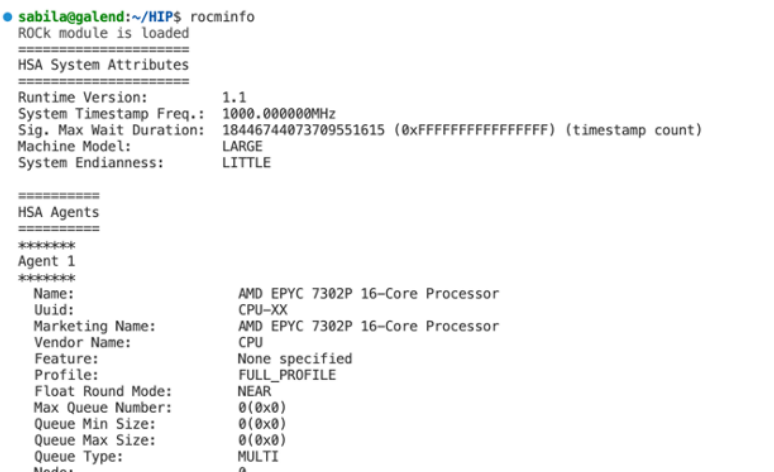
\includegraphics[width=0.75\linewidth]{FileAusiliari/Screenshots/Figure7-1.png}
    \caption{\bold{rocminfo}執行的截圖}
    \label{fig:rocminfo}
\end{figure}

如同我們稍早所講,rocminfo是個強大的工具可以讓開法者深入了解GPUs的功能及配置。\figref{fig:rocminfo} 展示了透過rocminfo獲得的一些寶貴的資訊。這豐富的資訊提供開法者有關GPUs的詳盡的細節,讓他們做出明智的決定、優化程式碼及微調應用程式以利用GPUs的特定功能及能力。

在ROCm生態系統中,每個HSAagent被指派一個獨一無二的識別符號,用於計算任務溝通及資源分配的便利。這個識別符號是通用又唯一的識別碼,區分每個agent系統中的彼此。我們更詳細的可以看範例截圖,如圖\figref{fig:HSA agent 1}。在這範例中,我們觀察到agent1被辨別為16個kernel的CPU設備。這些資訊讓開法者針對他們的程式碼去更有效的利用Agent 1的CPU資源,最佳化效能及有效執行任務。他能夠使開法者在GPU加速應用程式中,有關任務分配、資源利用和溝通策略做出的明智決定。

\begin{figure}
    \centering
    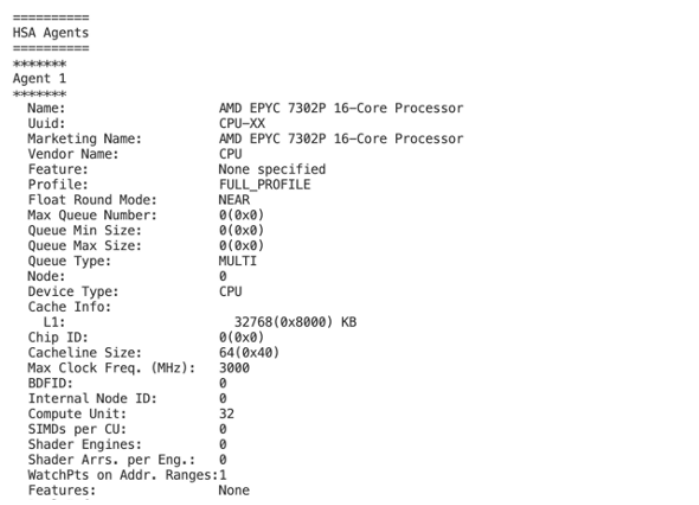
\includegraphics[width=0.75\linewidth]{FileAusiliari/Screenshots/Figure7-2.png}
    \caption{HSA agent 1 - 系統中的CPU}
    \label{fig:HSA agent 1}
\end{figure}

除了agent1,我們還有關於agent2寶貴的的資訊,如圖\figref{fig:HSA agent 2}。agent2被辨別為 Radeon Pro W6800 的 GPU 設備。這個GPU設備提供可以顯著的提升效能的強大能力。當檢查了 rocminfo 提供的資訊,我們發現Radeon Pro W6800 GPU包含3個級別的快取,即一個大小 16KB 的 L1 快取、一個大小 4MB 的 L2 快取及一個 大小 128MB 的 L3 快取。這些快取扮演至關重要的角色去減少記憶體存取的延遲及提升整體效能,因為其儲存頻繁訪問的資料在更靠近CUs的位置。除此之外,Radeon Pro W6800 GPU 有60個 CUs ,使其成為強大的計算設備。每個計算單元包含 60 個 SIMD 單元。這個硬體架構設計允許 GPU 在每個計算單元使用相同的指令,同時執行最多 60 個操作在獨立的資料上。這種平行化的能力顯著提高效計算密度任務的能力。Radeon Pro W6800 GPU 的 wavefront 大小是32,代表 32 個 thread 可以平行化執行在每個 CUs 上。這種thread平行執行使 GPU 能夠同時處理多個thread,提升吞吐量並加速執行可平行化的工作負載。

了解 Radeon Pro W6800 GPU 的這些技術細節可以讓開發者深入了解這款高效能設備的底層架構和功能。利用這些知道,開發者可以優化他們的 GPU 加速應用程式,確保有效利用 GPU 資源以達到最大效能。

\begin{figure}
    \centering
    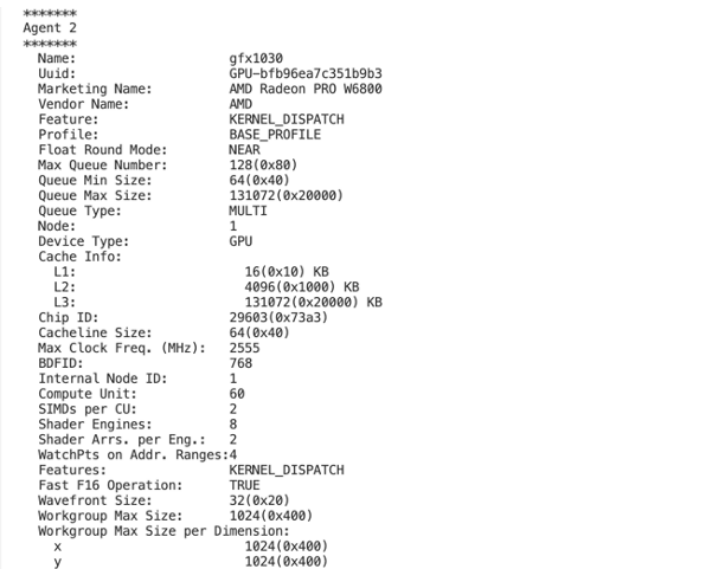
\includegraphics[width=0.75\linewidth]{FileAusiliari/Screenshots/Figure7-3.png}
    \caption{HSA agent 2 - 系統中的GPU}
    \label{fig:HSA agent 2}
\end{figure}

\section{\term{ROCm SMI}}

\term{ROCm SMI} 使系統管理員能夠追蹤多種系統階層的指標,例如電力、效能及溫度。通常,如果電腦上安裝了標準的 ROCm,\term{ROCm SMI}可以在 /opt/rocm/bin directory 找到。假定這個目錄已經在PATH的環境變數中,開發者可以打開終端機簡化輸入\term{rocm-smi}去訪問並監控多種系統層級與PCIe、電力管理、時脈、效能、錯誤及事件有關的參數。\term{ROCm SMI}也可以提供簡單的方法檢查\term{ROCm} kernel驅動程式,以確認是否正確地載入及確保所有系統GPUs適當的初始化。

執行 \bold{rocm-smi -h} 可以查看 \term{ROCm SMI} 版本的所有可用的功能列表,\bold{-h} 代表「幫助」。在這個部分,我們檢測該工具提供的功能,記住監控 GPU 資訊不需要管理員權限。然而,改變時脈頻率和功率狀態需要使用 \bold{sudo}。此外,可以執行 \bold{rocm-smi –showid}獲得 GPU ID,\bold{–showid} 讓使用者簡單地辨識和他們一起工作的GPU設備,這在多GPU系統特別有用,因為多GPU系統可能很難分辨不同的設備。

除了提供GPU設備的資訊,\bold{ROCm SMI}也允許使用者監控變動的硬體真實時間。透過使用 \bold{watch -n0 rocm-smi} 指令,可以獲得隨隨真實時間變動的GPU 溫度和平均消耗功率。在這 \bold{watch} 是個標準的 Linux 指令,而 n0 代表盡可能最小執行 \bold{rocm-smi} 指令的間隔時間。這特色在監控效能和辨識任何在操作過程可能遇到的問題或異常現象特別有用。

\term{ROCm SMI}通常用來看系統動態資訊,如同圖\figref{fig:Output of the ROCm SMI tool}。這輸出來自於本書開發的系統。擁有8張GPUs(0-7),每個設備的 GPU 頻率設定為 800 MHz,而記憶體頻率設定 1,600 Mhz。因為系統閒置,GPU 顯示隨機存取記憶體(VRAM)和使用率百分比都為0\%。"perf" 列顯示 "auto",代表動態功耗管理 (DPM) 的功能已經啟動,DPM 模組根據系統的工作負載需求和功率限制自動調整電壓和頻率。此外,可以用 \bold{rocm-smi}改變 GPU 設定。我們注意到在\figref{fig:Output of the ROCm SMI tool},效能等級預設為auto(自動)。要修改這個,我們可以使用\bold{rocm-smi –setperflevel low} 指令去設定效能等級為低。透過這調整,我們可以更好根據特定需求優化 GPU 效能,從而顯著提升工作負載的效率。

使用 \bold{rocm-smi –showsclkrange} 可以查詢 GPU 時脈頻率的列表,記憶體時脈頻率的列表則可以用 \bold{rocmsmi –showmclkrange} 查詢。超級使用者權限的使用者可以改變時脈參數。例如, \bold{–setclk} 用來改變圖形時脈,\bold{–setmclk} 用來改變記憶體時脈。注意在不同 GPU 系統有關改變時脈行為提供不同程度的靈活性。因此,假如你的系統並不支援特定的設定,\term{ROCm SMI}會回傳\bold{NOT\_SUPPORTED}。

另一個有用的 \term{ROCm SMI} 指令是 \bold{–showtopo},呈現節點的拓譜圖。程式設計者可以在多 GPU 系統上利用該資訊了解不同 GPU 內部是如何連接的(例如:PCIe 或 AMD 的晶片間全域記憶體的互聯)。這指令也提供 GPUs 間的距離,以跳數表示一個 GPU 到另一個 GPU。這在多GPU系統中可以用來優化的溝通模式。

\begin{figure}
    \centering
    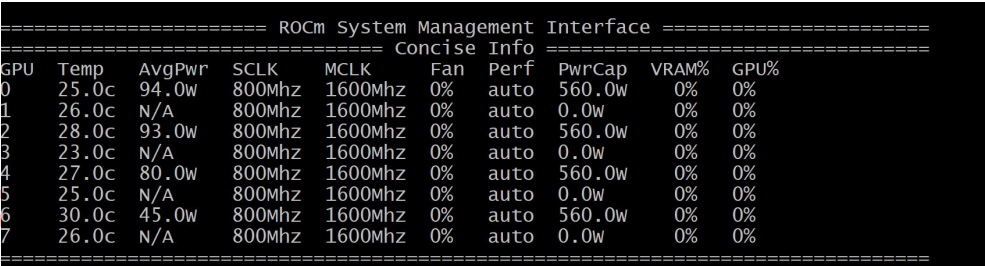
\includegraphics[width=0.75\linewidth]{FileAusiliari/Screenshots/Figure7-4.png}
    \caption{\term{ROCm SMI}工具的輸出}
    \label{fig:Output of the ROCm SMI tool}
\end{figure}

假如一個程式設計者想要在程式裡使用 \term{ROCM SMI} 而不是用 CLI,需要使用 \term{ROCm-SMI-Lib} 提供直接的 C/C++ 圖形化的使用者介面,此開源的函式庫可以在Github \cite{ROCm-SMI-Lib} 找到。目前支援APIs的集合寫在rocm\_smi.h的標頭檔中。

\lstref{lst:ROCm-SMI-Lib} 給了一個可以存取 \term{ROCm SMI} 函式庫的程式範例。程式碼的迴圈透過使用者系統的所有 AMD GPUs 並印出每個 GPU 獨特的 PCI \bold{domain:bus:device:function} 辨識碼。常規的初始化 \term{ROCm-SMI-Lib} 和決定在系統中 ROCm 設備的數字。接著,使用迴圈,程式碼取回每個設備的 PCI 連接 \bold{domain:bus:device}。顯示完這些資訊後,程式呼叫 \term{rsmi\_shut\_down} 執行在程式結束前必要的清理。範例中有功能上的更多細節,請參考函式庫的標頭檔,\term{rocm\_smi.h},它是開源儲存庫~\cite{ROCm-SMI-Lib}的一部分。

命令列工具和 API 層級呼叫都有他們的使用時機。假如想要在應用程式裡本身包含有關時脈頻率、測量隨時間變化的功率的程式碼,API 層級呼叫非常有用。通常用於擴展基準實驗,避免測量時需要查看 \term{ROCm SMI} 命令列工具的輸出。

\begin{lstlisting}[language=C, caption={\term{ROCm-SMI-Lib}範例}, label={lst:ROCm-SMI-Lib}]
#include <stdio.h>
#include <stdint.h>
#include "rocm_smi/rocm_smi.h"

int main() {
    rsmi_status_t ret;
    uint32_t num_devices;
    uint64_t bdf;

    // Return code checks are skipped for clarity.
    ret = rsmi_init(0);
    ret = rsmi_num_monitor_devices(&num_devices)

    for (int i=0; i < num_devices; ++i) {
        ret = rsmi_dev_pci_id_get(i, &bdf);
        printf("Device[%d] : PCI:%04lX:%02lX:%02LX:%02LX\n", i,
                        (bdf >> 32) & 0xffffffff, (bdf >> 8) & 0xff,
                        (bdf >> 3) & 0x1f, bdf & 0x7);
    }
    ret = rsmi_shut_down();
    return 0;
}
\end{lstlisting}

\section{\term{ROCm} 除錯器}
\label{sec:7.3}

設計良好除錯器對於 GPU 程式設計者的支援置關重要。假如在運行時應用程式產生意外結果或崩壞,逐行執行kernel將有助於辨識問題的根源。除錯器是檢測每個thread暫存器內容或檢視參數值的重要工具。為了這些目的,ROCm提供 \term{rocgdb} 除錯器,基於一個通常用在CPU應用程式除錯的工具\term{GDB}之上建造。

在這段落,我們學習如何有效使用 \term{rocgdb} 除錯及印出 wavefront 資訊。在範例 kernel 中每個 thread 從輸入數組讀取一個元素,多個 thread 透過他們的 thread ID 並儲存結果在輸出數組。輸入數組的值初始化成第i個元素包含值i。採用這簡單的協定,索引0包含一個0,索引1包含一個1,以此類推。在一開始kernel執行,我們計算值行緒ID以獲得輸入和輸出數組的起始位置。在\lstref{lst:Scalar multiply kernel} 的第18行,我們讀\bold{a}數組和thread ID。然後我們將它們相乘並將結果儲存在\bold{c}陣列中。在我們的範例中,我們使用256 thread,每個工作群組大小為64。因此,總共有4個工作群組,每個工作群組有64個thread。

我們的範例在每個 wavefront 有 64 個 thread 的 AMD GPU 上編譯並執行的。記得總共有4個wavefront是很重要的。注意展示到目前為止thread概念與“\term{GDB} threads”的差異。一個\term{GDB} threads可以代表一個主機端 OS 在執行時產生的thread,或是特定於wavefront映射到特定的\term{GDB} thread。因此,如果我們關注在設備端的\term{GDB} threads,其只有四個,因為我們的樣本執行總共有四個wavefront。在下面的例子,當提及 “threads”和 “thread IDs”代表實際上運行在GPU的thread。明確地提及“debugger” threads 當作“GDB” threads。

要檢查wavefront暫存器的值為0,我們根據以下步驟:

\begin{enumerate}
    \item 在任何 GPU kernel除錯之前,我們必須使用\bold{-g}編譯選項來編譯程式,這樣除錯資訊就會被包在輸出的二進位檔。如同範例,我們運行\bold{hipcc -g scale\_hip.cpp -o scale\_hip},可以產生名子為\term{scale\_hip}的二進位檔。
    \item 現在,我們準備用\term{rocgdb}除錯,要啟動除錯環節,我們輸入\bold{rocgdb ./scale\_hip}。一旦進入除錯環境,我們從\term{GDB}環境的CLI運行程式。
    \item 我們在kernel的第19行設定斷點,這行是輸出結果計算出來的地方。要使用\term{GDB} CLI設定斷點,我們輸入\bold{break scale\_hip.cpp:19}。接著,我們繼續使用\term{GDB}指令執行,\bold{c}(也就是發出繼續執行的指令)。當所有wavefront依據相同的控制流,每個wavefront將撞擊到這個斷點。
    \item 設定多個斷點後,我們可以在每個斷點分析程式狀態和深入了解他的邏輯。一旦斷點被放置,我們可以在GDB的指令介面使用\bold{info b}指令去顯示我們設定的斷點其狀態和細節。細節資訊包含有設定多少斷點、提供每個設定斷點的原始程式碼行數和為一個數字的斷點ID。
    \item 要開始除錯,我們可以使用\bold{r}(運行)指令用指定的斷點開始執行程式,並在第一次遇到的斷點時暫停執行。
    \item 在到達斷點後,\bold{c}(繼續)指令使我們能夠從現在的斷點恢復執行程式。一旦使用這指令,除錯器執行程式直到碰到下個斷點則會再次暫停。這工能能夠更大步數執行程式碼對分析程式在不同階段的行為很有用。
    \item 接著,我們使用\bold{info threads}查看當前活動thread的列表。輸出結果如同在\lstref{lst:Output of info threads command}。回想一下,我們在這討論的是\term{GDB} threads,不要將其與在GPU運行上的threads混淆。\term{GDB} threads IDs為1、2和3是由作業系統產生的host-side threads。Thread IDs為5、6、7和8指的是四個wavefronts被kernel啟動。星號下一個\term{GDB} Thread 5表示wavefront碰到斷點。
    \item 接下來,我們需要檢查當前在斷點執行的程式碼。假如我們在CPU除錯,我們可能會使用’l’或'list'指令去檢查程式碼。相同的應用到GPU程式。然而,由於GPU二進位檔經過最佳化,可能並不容易辨識組合程式碼在哪裡執行或變數如何映射到暫存器。因此,GPU除錯通常在組合階段完成。假如讀者不熟悉AMD GPU的組合語言,請參考\chapref{chap:AMD_GPU_internal}詳細的介紹。要檢查組合語言,我們可以使用\bold{disassemble}指令。指令的輸出會是一系列的組合程式碼,組合程式碼由instructions的列表組成,每個由一個記憶體位置標記。
    \item 要檢查這個 wavefront 暫存器的值,我們輸入\term{GDB}指令\bold{info registers},印出與當前活動的thread有關的所有暫存器:在wavefront 0中,thread ID為。\lstref{lst:Partial output of info registers command}顯示這指令的部分輸出。有了這些資訊,程式設計者可以透過查看彙編級的kernel程式碼來驗證儲存輸出值的特定暫存器。在我們\bold{GDB}期間,可以使用\bold{disassemble scaleKernel}輕鬆的達到。

    繼續我們的範例,我們觀察到暫存器v3將值寫回去主記憶體之前儲存了最終結果。因此,透過檢查\lstref{lst:Partial output of info registers command}的第四行,我們可以看到暫存器v3的值在wavefront 0的所有64個thread。例如,第三個值是0x4,對應這個wavefront的thread ID 2。作為參考,thread ID 2從輸入數組\bold{a}載入值2,將其乘上thread ID的值2並輸出0x4。

    \item 繼續後,斷點會被其他的 wavefront 再次碰到。我們可以檢查 wavefront 裡額外暫存器的值。

\end{enumerate}

\begin{lstlisting}[language=C, caption={純量乘法kernel}, label={lst:Scalar multiply kernel}]
#include "hip/hip_runtime.h"
#include <stdio.h>
#include <stdlib.h>
#include <math.h>
#define HIP_ASSERT(x) (asert((x)==hipSuccess))

// HIP kernel. Each thread takes care of one element of c
__global__ void scaleKernel(int *a,int *c, int n)
{
    // Get our global thread ID
    int id = blockIdx.x*blockDim.x+threadIdx.x;
    // Make sure we do not go out of bounds
    if (id < n)
    {
    
        c[id] = id*a[id];
    }
}
\end{lstlisting}

\begin{lstlisting}[language=bash, caption={info threads指令的輸出}, label={lst:Output of info threads command}]
Id Target Id Frame
1 Thread 0x7ffff7fdc880 (LWP 58984) "a.out" 0x00007ffff5fc9ef7 in sched_yield () from /lib/x86_64-linux-gnu/libc.so.6
2 Thread 0x7ffff4f9e700 (LWP 58990) "a.out" 0x00007ffff5fdc317 in ioctl () from /lib/x86_64-linux-gnu/libc.so.6
4 Thread 0x7ffff4573700 (LWP 58992) "a.out" 0x00007ffff5fdc317 in ioctl () from /lib/x86_64-linux-gnu/libc.so.6
* 5 AMDGPU Thread 2:1:1:1 (0,0,0)/0 "a.out" scaleKernel (a=<optimized out>, c=<optimized out>, n=<optimized out>) at vadd_hip.cpp:20
6 AMDGPU Thread 2:1:1:2 (1,0,0)/0 "a.out" scaleKernel (a=<optimized out>, c=<optimized out>, n=<optimized out>) at vadd_hip.cpp:20
7 AMDGPU Thread 2:1:1:3 (2,0,0)/0 "a.out" scaleKernel (a=<optimized out>, c=<optimized out>, n=<optimized out>) at vadd_hip.cpp:20
8 AMDGPU Thread 2:1:1:4 (3,0,0)/0 "a.out" scaleKernel (a=<optimized out>, c=<optimized out>, n=<optimized out>) at vadd_hip.cpp:20
\end{lstlisting}

\begin{lstlisting}[language=bash, caption={info registers的部分輸出}, label={lst:Partial output of info registers command}]
v0          {0xe8202000, 0xe8202004, 0xe8202008, 0xe820200c, 0xe8202010, 0xe8202014, 0xe8202018, 0xe820201c, 0xe8202020, 0xe8202024, 0xe8202028, 0xe820202c, 0xe8202030, 0xe8202034, 0xe8202038, 0xe820203c, 0xe8202040, 0xe8202044, 0xe8202048, 0xe820204c, 0xe8202050, 0xe8202054, 0xe8202058, 0xe820205c, 0xe8202060, 0xe8202064, 0xe8202068, 0xe820206c, 0xe8202070, 0xe8202074, 0xe8202078, 0xe820207c, 0xe8202080, 0xe8202084, 0xe8202088, 0xe820208c, 0xe8202090, 0xe8202094, 0xe8202098, 0xe820209c, 0xe82020a0, 0xe82020a4, 0xe82020a8, 0xe82020ac, 0xe82020b0, 0xe82020b4, 0xe82020b8, 0xe82020bc, 0xe82020c0, 0xe82020c4, 0xe82020c8, 0xe82020cc, 0xe82020d0, 0xe82020d4, 0xe82020d8, 0xe82020dc, 0xe82020e0, 0xe82020e4, 0xe82020e8, 0xe82020ec, 0xe82020f0, 0xe82020f4, 0xe82020f8, 0xe82020fc}
v1          {0x7fff <repeats 64 times>}
v2          {0x0 <repeats 64 times>}
v3          {0x0, 0x1, 0x4, 0x9, 0x10, 0x19, 0x24, 0x31, 0x40, 0x51, 0x64, 0x79, 0x90, 0xa9, 0xc4, 0xe1, 0x100, 0x121, 0x144, 0x169, 0x190, 0x1b9, 0x1e4, 0x211, 0x240, 0x271, 0x2a4, 0x2d9, 0x310, 0x349, 0x384, 0x3c1, 0x400, 0x441, 0x484, 0x4c9, 0x510, 0x559, 0x5a4, 0x5f1, 0x640, 0x691, 0x6e4, 0x739, 0x790, 0x7e9, 0x844, 0x8a1, 0x900, 0x961, 0x9c4, 0xa29, 0xa90, 0xaf9, 0xb64, 0xbd1, 0xc40, 0xcb1, 0xd24, 0xd99, 0xe10, 0xe89, 0xf04, 0xf81}
v4          {0x7fff <repeats 64 times>}
v5          {0x7fff <repeats 64 times>}
\end{lstlisting}

正如我們所見,\term{rocgdb} 使我們能夠透過設定斷點並逐個斷點跳轉去除錯 GPU kernels。我們可以檢索每個斷點詳細的運行資訊,包含在 wavefront 裡暫存器的細節。

\section{\term{ROCm} 分析器}

每當談到最佳化GPU效能,分析和追蹤是兩個必要的工具,可以幫助開法人員深入了解他們的應用程式如何利用GPU設備。ROCm提供兩個強大的工具幫助分析和追蹤:\term{ROCTracer}和\term{rocprofiler}。

\subsection{ROCTracer}

\term{ROCTracer}用來評估應用程式的效能,而且GPU分析模式可以提供我們來自GPU硬體效能計數器的更詳細測量。\term{ROCTracer}透過追蹤應用程式的執行和測量每個函數或程式碼的區塊執行花費時間來評估應用程式效能。\term{ROCTracer}旨在幫助開發人員辨識花費最多時間的程式碼部分。那麼,程式設計師可以專注於最佳化程式碼這耗時的部分。為了執行應用程式追蹤,我們有很多可用的選項。系統架構包含底部的硬體、作業系統,例如在中間的 AMD KFD 驅動程式、一個介面例如 HSA 及最上層 HIP 的執行。我們可以在不同層級執行應用程式追蹤。例如,假如使用\bold{–hip-trace}選項,我們將可以追蹤 HIP 運行所在的使用者層級。使用\bold{–hsa-trace}選項將能夠追蹤 HSA 層級。使用\bold{–kfd-trace}選項,我們將能夠在AMD KFD 驅動程式層級進行追蹤。通常,追蹤較高層級允許使用者輕易追蹤結果連結到有關程式碼,或辨別問題發生原因的結果。透過追蹤較低階層,我們可以獲得有關效能問題更詳細的資訊。

要用\term{ROCTracer}追蹤執行應用程式,我們可以根據我們想要追蹤的應用程式二進位檔,使用\bold{rocprof –hiptrace <your\_application>}指令。使用這個指令,程式設計者將生成4個輸出檔案,包含有關應用程式執行的資訊。檔案\term{results.copy\_stats.csv}(\lstref{lst:results.copy_stats.csv output})紀錄每個hip運行時呼叫的時間測量值,資料以CSV格式呈現。這包含在設備和主機執行記憶體複製的操作所花費執行時間的部分,資料以奈秒為單位顯示。

\begin{lstlisting}[language=bash, caption={應用程式追蹤模式下\term{results.copy\_stats.csv}的輸出}, label={lst:results.copy_stats.csv output}]
"Name","Calls","TotalDurationNs","AverageNs","Percentage"
"CopyDeviceToHost",2,9654400,4827200,81.6235566612597
"CopyHostToDevice",2,2173558,1086779,18.376443338740298
\end{lstlisting}

檔案\term{results.hip\_stats.csv}(\lstref{results.hip_stats.csv output})總結執行時間,並按API細分。除了我們稍早討論的APIs,這個檔案也包含三個APIs的執行時間,分別為\term{hipLaunchKernel}、\term{\_\_hipPushCallConfiguration} 及 \term{\_\_hipPopCallConfiguration}。這三個函數是每次kernel啟動時,三角括號語法相關的實際API呼叫。當我們初始化一個kernel啟動,HIP將會傳送呼叫設定給GPU,包含kernel的維度、流、本地記憶體大小和kernel參數,讓GPU呼叫\_\_hipPushCallConfiguration API。根據這個,\term{hipLaunchKernel}指令觸發kernel的執行。最終,\term{\_\_hipPopCallConfiguration}負責清除kernel的相關資訊,使下個kernel可以有乾淨的設定檔啟動。

\begin{lstlisting}[language=bash, caption={應用程式追蹤模式下\term{results.hip\_stats.csv}的輸出}, label={results.hip_stats.csv output}]
"Name","Calls","TotalDurationNs","AverageNs","Percentage"
"hipMemcpy",4,537814533,134453633,99.25629643299268
"hipDeviceSynchronize",1,2834079,2834079,0.5230431088750803
"hipLaunchKernel",1,766035,766035,0.141375497262822228
"hipMalloc",3,246963,82321,0.04557822675271806
"hipFree",3,125437,41812,0.02315001044359153
"hipEventRecord",2,34503,17251,0.00636769701392124
"hipEventElapsedTime",1,6146,6146,0.0011342742905706734
"__hipPushCallConfiguration",1,5727,5727,0.0010569457959808406
"hipEventCreate",2,5238,2619,0.0009666984598127542
"hipEventSynchronize",1,2794,2794,0.0005156463338520113
"__hipPopCallConfiguration",1,2793,2793,0.0005154617789723219
\end{lstlisting}

還有另一個輸出檔案稱為\term{results.stats.csv}(\lstref{lst:results.stats.csv output})。這檔案匯總了kernel的執行時間。最終,除了匯總資料,我們想要一個更詳細的細分資料版本。在這個範例中,我們有檔案\term{results.json}。雖然這個檔案對人來說是可讀的(需要花精力),但可以更容易透過視覺化追蹤去了解執行過程。檔案\term{results.json}根據標準追蹤格式,使我們能夠使用chrome追蹤工具來視覺化執行追蹤。我們首先在 Chrome 瀏覽器中輸入 \url{chrome://tracing},接著將我們的json檔上傳至該頁面。然後我們可以視覺化追蹤內容了。

\begin{lstlisting}[language=bash, caption={應用程式追蹤模式下\term{results.stats.csv}的輸出}, label={lst:results.stats.csv output}]
"Name","Calls","TotalDurationNs","AverageNs","Percentage"
"vector_add(float*, float*, float*, int)",1,2850719,2850719,100.0
\end{lstlisting}

\subsection{rocprofiler}

如同先前所提,在kernel執行時,\term{rocprof}允許程式設計者取得硬體計數器的分析資訊。這計數器的值可以幫助程式設計者更好了解,如何在各種基於軟體的優化上提升硬體使用率。\term{rocprof}產生快取擊中和失誤、不同形式的指令執行的頻率、等待記憶體指令完成所花費的時間和其他有關效能關鍵資訊的統計。分析器還可以針對群體裡的kernel做選擇性的分析規則,或甚至特定kernel的呼叫。

注意GPU硬體計數器的數字和在GPU架構上的不同。嘗試優化應用程式效能的第一步是使用\bold{rocprof –list-basic}取得GPU硬體計數器的詳細資訊。輸出會包含基礎硬體計數器的列表。除此之外,\bold{rocProf –list-derived}顯示分析器所產生的指標,由基礎硬體計數器收集。程式設計者可以選擇取得特定的集合去量化分析瓶頸。這件事是非常重要的,因為每個GPU在單次傳遞可以收集到的計數器數量有限制。當程式設計者指定大量效能計數器進行分析時,硬體會重複執行去收集資訊,最終導致增加分析時間。\term{rocProf}支援兩種模式:i)效能分析,測量kernel執行時間,和 ii)效能計數器,收集指定硬體計數器的資料。

接著,我們考慮一個使用在\chapref{chap:getting_started_with_hip_programming} 開發的\term{vector\_add} kernel的分析範例。我們使用\term{hipcc}編譯我們的應用程式產生輸出二進位檔,\term{vadd}。我們一開始使用效能分析模式,因為我們想要收集kernel執行時間。藉由運行\bold{rocprof –stats <your\_application>}完成,它的輸出檔,\term{results.stats.csv},如圖\lstref{lst:rocProf output} 所示。在這
逗號分隔值(CSV)檔案裡的資訊包含統計數據,像是kernel 被呼叫的次數(其中一個在我們的範例)、全部和平均以奈秒計數的kernel執行時長(5,920 ns 為 vadd)以及kernel花費GPU應用程式全部總量的比例(在我們的範例為100\%,因為只有一個kernel)。這些效能分析測量有助於辨識應用程式中活動的kernel,並提供每個kernel在所運行時的分類。這些資訊將幫助程式設計者,使他們能夠縮小大多數kernel執行時間的集合。

\begin{lstlisting}[language=bash, caption={效能測量模式中\term{rocProf}的輸出}, label={lst:rocProf output}]
"Name","Calls","TotalDurationNs","AverageNs","Percentage"
"vecAdd(double*, double*, double*, int) [clone.kd]",1,5920,5920,100.0
\end{lstlisting}

然後,我們透過使用效能計數器模式的範例,展示如何收集效能硬體計數器。\lstref{lst:rocProf input file}顯示範例輸入檔,\term{input.txt}。第一行包含"pmc",指定我們分析運行時希望收集的計數器。在這範例中,我們收集\bold{TCC\_EA\_RDREQ\_sum}和\bold{TCC\_EA\_WRRREQ\_sum}。這些計數器計算讀取及快取與主記憶體發生寫入分別的次數。第二行指定我們希望分析的呼叫範圍。在這個案例中,我們只有一個呼叫;因此,我們指定0:1。假如我們在應用程式啟動這個kernel許多次,雖然只對分析特定呼叫感興趣,我們可以相對應指定該細節。例如,假如我們想要分析100次中的第55次呼叫,我們只需指定”55”。從第55次開始分析接下來的所有呼叫,我們設定範圍為”55:”。第三行,“gpu”,指定我們希望分析的GPU ID。在多GPU系統,這數字可以相對應的設定,取決於討論的GPU。最後一行是“kernel”行,指定kernel名稱。要分析多個kernel,我們使用逗號分隔符。在這範例,我們只解決單一kernel,\term{vecAdd}。當有我們的輸入檔,我們準備好去分析我們的\term{vector\_add} kernel。要分析它的執行,我們用\bold{rocprof -i input.txt -o vadd\_profile.csv ./vadd}傳遞輸入文字檔給分析器,觸發 \term{rocProf},分析所需的指標。最後的輸出結果存在 \term{vadd\_profile.csv},如圖\lstref{lst:rocProf output file for the vectorAdd kernel}所示。回想一下,這個名稱是我們使用\bold{-o}的參數,傳遞給\term{rocprof}。輸出檔包含許多不同的值,像是 kernel 名稱、process ID 和暫存器使用。接近文件尾端,我們將找到兩個分析指標的結果:\bold{TCC\_EA\_RDREQ\_sum}和\bold{TCC\_EA\_WRREQ\_sum}。它們輸出分別為 “2610” 和 “1280”,因為這個 kernel 讀取次數是寫入次數的兩倍(也就是\term{vadd}讀取\bold{a}和\bold{b}與寫入\bold{c})。

\begin{lstlisting}[language=bash, caption={vectorAddkernel的\term{rocProf}輸入檔}, label={lst:rocProf input file}]
pmc: TCC_EA_RDREQ_sum, TCC_EA_WRREQ_sum
range: 0:1
gpu: 0
kernel: vecAdd
\end{lstlisting}

\begin{lstlisting}[language=bash, caption={vectorAddkernel的\term{rocProf}輸出檔}, label={lst:rocProf output file for the vectorAdd kernel}]
Index,KernelName,gpu-id,queue-id,queue-index,pid,tid,grd,wgr,lds,scr,vgpr
,sgpr,fbar,sig,obj,TCC_EA_RDREQ_sum,TCC_EA_WRREQ_sum
0,"vecAdd(double*, double*, double*, int) [clone .kd]"
,0,0,0,15239,15242,10240,256,0,0,12,24,0,0x0,0x7f9ba4c45800,2610,1280
\end{lstlisting}

現在我們已經學會如何使用 \term{rocprof} 分析器,在下個章節,我們將分析及優化整個 GPU 應用程式。回想一下,分析器的目標是提供程式設計者有用的資訊,使其能夠針對性的優化。

\section{\term{ROCm} 分析器 V2}

ROCm分析器的第二個版本隨 ROCm 6.0 推出,是 \bold{rocprof} 的不向後相容更新。由於與早期版本不相容,兩個版本在標準的 ROCm 安裝共同存在:\bold{rocprof} v1和它的接替者。與 rocprof v1 類似,rocprof v2 也支援應用程式追蹤和 kernel 分析模型。

\subsection{應用程式追蹤}

使用 rocprofv2 和各種追蹤選項來追蹤HIP/HSA API、非同步化的活動和 kernel 的調度。這些追蹤選項將顯示如下。注意這些指令尚未產生輸出,我們需要輸入插件(很快會介紹)去產生輸出。

\begin{lstlisting}[language=bash, caption={使用rocprofv2應用程式追蹤功能要使用的指令}, label={lst:trace feature of rocprofv2}]
# HIP API & asynchronous activity tracing
rocprofv2 –hip-api <app_relative_path>
rocprofv2 –hip-activity <app_relative_path>

# HSA API & asynchronous activity tracing
rocprofv2 –hsa-api <app_relative_path>
rocprofv2 –hsa-activity <app_relative_path>

# Kernel dispatches tracing
rocprofv2 –kernel-trace <app_relative_path>

# HIP & HSA API and asynchronous activity and kernel dispatches tracing
rocprofv2 –sys-trace <app_relative_path>
\end{lstlisting}

rocprofv2 命令列介面支援追蹤在HIP和HSA兩種層級的APIs。通常來說,HIP APIs直接訪問使用者程式。它讓分析HIP追蹤更加簡單,因為使用者可以直接追蹤映射到的程式。HSA API追蹤更加適合想要了解低層級硬體行為的進階用戶。

HIP 和 HSA APIs都支援非同步行為(也就是非同步記憶體複製)。假如選擇 –hip-api 或 –hsa-api,追蹤將只會紀錄API執行時間,但不包含相關動作(例如:記憶體複製)發生的時間。要記錄真實的動作時間,可以使用 –hipactivity 和 –hsa-activity 選項。除此之外,要記錄 kernel 執行,rocprofv2 命令列介面提供專用的 –kernel-trace 選項。

在一個分析運行時,很多個追蹤選項可以同時使用。為了簡化指令,使用者可以使用 –sys-trace 指令,它包含上述提及的所有追蹤。

rocprofv2 命令列介面使用模組化的插件系統來讓使用者選擇分析輸出格式。ROCProfilerV2 附隨的插件和輸出格式的描述列在 Table \ref{tab:plugins}。

\begin{table}[htbp]
    \centering
    \begin{tabular}{p{4cm}p{10cm}}
        \toprule
        \multicolumn{1}{c}{插件} &
        \multicolumn{1}{c}{輸出格式} \\
        \midrule
        File & 文字檔 (.txt) \\
        Perfetto & Protobuf,採用 Chromium 專案追蹤事件格式 \\
        Advanced Thread Tracer &  二進位檔,用於視覺化分析工具 \\
        CTF & 二進位檔,採用CTF格式,可供Babeltrace等公共工具使用 \\
        OTF2 & 二進位檔,採用開放式追蹤格式版本2(OTF2),此追蹤可以被Score-P 、 TAU 和 Vampire等工具使用。 \\
        \bottomrule
    \end{tabular}
    \caption{rocprofv2支援的插件}
    \label{tab:plugins}
\end{table}

要生成輸出,變數 \bold{OUTPUT\_PATH} 必須設成所需的目錄。否則,不會產生輸出。唯一一個例外是檔案插件,如果 \bold{OUTPUT\_PATH} 不存在,它會將追蹤轉成標準輸出。

有鑑於 rocprofv2 命令列介面支援 Perfetto 輸出格式,使用者可以簡單用 Perfetto 視覺化執行追蹤。要使用 Perfetto,打開\url{https://ui.perfetto.dev},從左邊的導航列選擇 “Open trace file”,和選擇追蹤去視覺化。

下圖為從 Perfetto 介面的截圖。任務以甘特圖風格,x 軸表示時間且每個三角形表示任務開始及結束的時間。任務按行排列。在這我們有HIP API、HSA API、一個佇列和一個流。

\subsection{kernel 分析}

應用程式的追蹤功能允許使用者評估 kernel 的執行時間,但卻沒提供有關 kernel 為何花費時間這麼長的資訊。為了調查,使用者將需要使用 kernel 分析功能去深入調查 kernel 執行。kernel 分析功能允許使用者收集由硬體收集的效能指標。

要檢查支援效能計數器和指標,rocprofv2 命令列介面提供–list-counters 選項,輸出將包含指標的列表像是下面的範例。

\begin{figure}
    \centering
    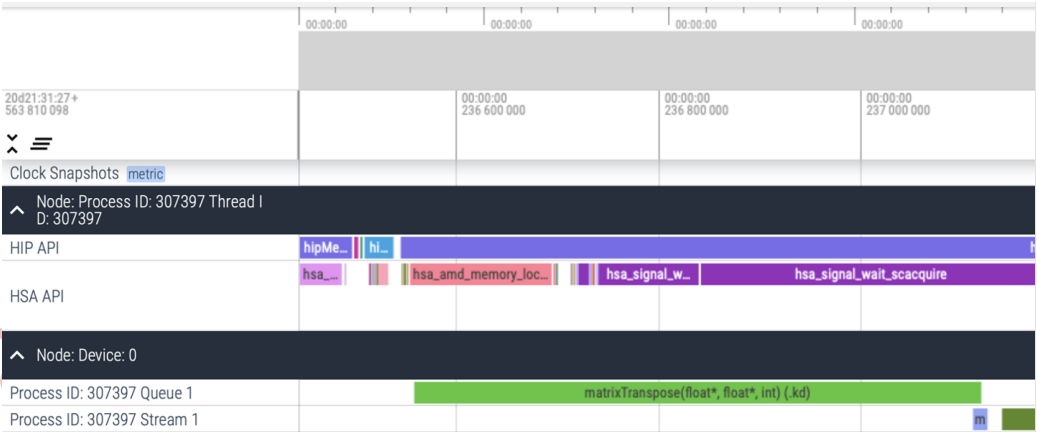
\includegraphics[width=1\linewidth]{FileAusiliari/Screenshots/Figure7-5.png}
    \caption{使用 Perfetto 視覺化 rocprofv2 取得的應用程式追蹤}
    \label{fig:captured application trace}
\end{figure}

\begin{lstlisting}[language=bash, caption={rocprofv2計數器的範例}, label={lst:rocprofv2 counter}]
gfx1030:0 : SQ_WAVES
: Count number of waves sent to SQs. {emulated, global, C1}
block SQ can only handle 8 counters at a time
\end{lstlisting}

這些條目可以理解如下:
\begin{enumerate}
    \item Gfx1030: GPU 架構
    \item 0: GPU ID。目前的機器可能有多個GPUs。
    \item SQ\_WAVES: 計數器名稱。通常,第一個底線之前的標記是 GPU 區塊的名稱。在這裡,SQ是個區塊負責管理 wavefronts 和發出指令。
    \item Count number …: 計數器的描述
    \item Block SQ …: 使用效能計數器的硬體限制。每個SQ有8個計數器。因此我們在一次運行不能收集太多指標。
\end{enumerate}

要使用 rocprofv2 去收集硬體計數器和衍伸的指標,可以使用 -i 選項提供輸入檔。

\begin{lstlisting}[language=bash, caption={使用rocprofv2分析kernel的指令}, label={lst:profile kernels with rocprofv2}]
rocprofv2 -i samples/input.txt <app_relative_path>
input.txt
\end{lstlisting}

輸入文件是個文字檔,提供rocprofv2進行計數器和指標收集。它通常由四個部分組成,即要使用的效能計數器、分析的GPUs、分析的kernel名稱和分析kernel的範圍。除了pmc以外的欄位都是可選擇的。

\begin{lstlisting}[language=bash, caption={rocprofv2kernel分析功能的輸入檔}, label={lst:Input file for kernel profiling feature of rocprofv2}]
pmc: SQ_WAVES TA_UTIL
range: 0:1
gpu: 0
kernel: matrixTranspose
\end{lstlisting}

輸入檔中的欄位描述如下:
\begin{itemize}
    \item PMC: 文字檔中以 ”pmc” 開頭的行是使用者感興趣收集的指標群組。可以用 –list-counters 選項產生的輸出選擇效能計數器。

    一次運行分析可以收集的指標數量被 GPU 硬體資源限制。假如太多指標被收集,kernel需要執行多次去收集指標。對於多次執行的情況,在輸入檔包含多行的 pmc。每次運行 kernel 都可以收集每個 pmc 行中的指標。
    \item GPU: 以關鍵字 gpu 開頭的行指定要收集硬體計數器的 GPU(s) 。這能夠支援分析多個 GPUs 。你可以以逗號分隔指定多個GPUs,例如:gpu: 1,3。
    \item Kernel: 以關鍵字 kernel 開頭的行指定需要進行分析的 kernel 名稱。
    \item Range:  以關鍵字 range 開頭的行指定 kernel 調度的範圍。指定範圍有助於在應用程式發生多 kernel 調度及使用者想要選擇特定 kernel 調度的情況。在上面的例子,範圍0:1表示對一個 kernel 進行分析。
\end{itemize}

rocprofv2 命令列介面在輸出中,報告每個 kernel 每個指標的一個值。按照輸出格式,使用者仍然可以使用插件去控制輸出格式。這裡我們將重點放在檔案輸出和 Perfetto 的輸出。

檔案插件為每個kernel產生新的資料條目(見以下範例)。對於每個kernel,基礎資訊(例如:gpu\_id、sgpr count等等)條列在指定的使用者效能計數器之前。每個值條列以“值的名稱(值)”的格式。

\begin{lstlisting}[language=bash, caption={rocprofv2kernel分析功能的輸出檔}, label={lst:Output of kernel profiling feature of rocprofv2}]
dispatch[1], gpu_id(0), queue_id(1), queue_index(0), pid(320661), tid
(320661), grd(1048576), wgr(16), lds(0), scr(0), arch_vgpr(8),
accum_vgpr(0), sgpr(128), wave_size(32), sig(140670227584384), obj(1)
, kernel-name("matrixTranspose"), start_time(1811083228321204),
end_time(1811083228892614)
, SQ_WAVES (65536.000000)
, GRBM_COUNT (288690.000000)
, GRBM_GUI_ACTIVE (288690.000000)
, SQ_INSTS_VALU (1048512.000000)
dispatch[2], gpu_id(0), queue_id(1), queue_index(2), pid(320661), tid
(320661), grd(1048576), wgr(16), lds(0), scr(0), arch_vgpr(8),
accum_vgpr(0), sgpr(128), wave_size(32), sig(140670227584384), obj(2)
, kernel-name("matrixTranspose"), start_time(1811083230510950),
end_time(1811083231072480)
, SQ_WAVES (65552.000000)
, GRBM_COUNT (286162.000000)
, GRBM_GUI_ACTIVE (286162.000000)
, SQ_INSTS_VALU (1048704.000000)
\end{lstlisting}

使用者也可以使用 Perfetto 插件去產生可視化的輸出。以下是個當視覺化 kernel 分析輸出 Perfetto UI 的截圖。那有許多行。最後一行是kernel執行時間軸,和在應用程式追蹤模式使用 –kernel-trace 是一樣的。其他上面的行表示使用者選擇的效能計數器。

可視化提供了 kernel 執行時間以及效能指標的值在 kernel 中如何變化的良好概述。除此之外,使用者也可以藉由懸停或點擊條形圖獲取詳細值,以顯示效能指標的準確值。

\subsection{ROCSys}

作為 rocprofv2 的一部分,ROCSys 是個命令列工具,可以在追蹤或分析應用程式時控制效能分析工作階段(啟動/開始/停止/離開)。當運行長時間的工作負載(DNN 訓練),使用者可能希望在應用程式運行時控制應用程式並分析其中的一部分。ROCSys 允許在運行時開始/停止一個效能分析工作階段、分析結果和離開工作階段。使用者可以從一個終端機啟動工作階段及從另一個終端機使用 ROCSys 控制應用程式(開始/停止/離開)。

\begin{figure}
    \centering
    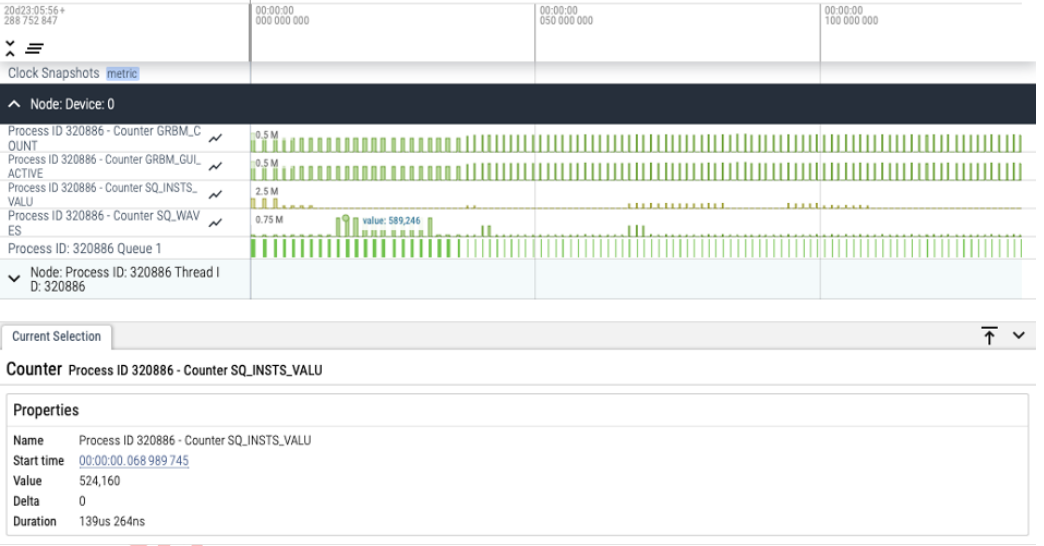
\includegraphics[width=1\linewidth]{FileAusiliari/Screenshots/Figure7-6.png}
    \caption{使用 Perfetto 視覺化 rocprofv2 獲得的kernel分析結果}
    \label{fig:captured kernel profiling results}
\end{figure}

接著,我們展示使用 ROCSys 的整個流程。

我們首先藉由呼叫 ROCSys 和 rocprofv2 建立一個工作階段。應用程式將會暫停直到 ROCSys 在第二步啟動工作階段 。

\begin{lstlisting}[language=bash, caption={使用 ROCSys 和 rocprofv2 建立工作階段}, label={lst:Creating a session using ROCSys and rocprofv2}]
/opt/rocm/bin/rocsys --session session1 launch rocprofv2 -i ../samples/
input.txt <long_running_app>
ROCSYS:: Session ID: 2109
ROCSYS Session Created!
ROCProfilerV2: Collecting the following counters:
- SQ_WAVES
- GRBM_COUNT
- GRBM_GUI_ACTIVE
- SQ_INSTS_VALU
- FETCH_SIZE
Enabling Counter Collection
\end{lstlisting}

第二,在另一個終端機視窗,使用者可以啟動工具工作階段。啟動工作階段將觸發應用程式運行。

\begin{lstlisting}[language=bash, caption={開始分析工作階段}, label={lst:Starting the profiling session}]
/opt/rocm/bin/rocsys --session session1 start
ROCSYS:: Starting Tools Session...
Dispatch_ID(1), GPU_ID(1), ... // All the metrics of a kernel
Dispatch_ID(2), GPU_ID(1), ... // All the metrics of a kernel
Dispatch_ID(3), GPU_ID(1), ... // All the metrics of a kernel
\end{lstlisting}

第三,我們也可以暫停工具工作階段。暫停分析工作階段之後,應用程式將會繼續執行。當我們執行任何 rocsys 指令,kernel 分析資訊將會轉到終端機。這些 kernel 會執行在當前和過去的指令。

\begin{lstlisting}[language=bash, caption={停止分析工作階段}, label={lst:Stopping the profiling session}]
/opt/rocm/bin/rocsys --session session1 stop
ROCSYS:: Stopping Tools Session...
Dispatch_ID(22397), GPU_ID(1), ... // All the metrics of a kernel
Dispatch_ID(22398), GPU_ID(1), ... // All the metrics of a kernel
Dispatch_ID(22399), GPU_ID(1), ... // All the metrics of a kernel
\end{lstlisting}

第四,停止分析工作階段後,我們可以重新啟分析工作階段,分析結果和重新啟動工具工作階段。

\begin{lstlisting}[language=bash, caption={重啟分析工作階段}, label={lst:Restarting the profiling session}]
/opt/rocm/bin/rocsys --session session1 start
ROCSYS:: Starting Tools Session...
Dispatch_ID(22400), GPU_ID(1), ... // All the metrics of a kernel
Dispatch_ID(22401), GPU_ID(1), ... // All the metrics of a kernel
\end{lstlisting}

最終,我們離開工具工作階段。一旦離開工作階段,我們將不能重啟。

\begin{lstlisting}[language=bash, caption={離開分析工作階段}, label={lst:Exiting the profiling session}]
/opt/rocm/bin/rocsys --session session1 exit
Dispatch_ID(16828), GPU_ID(1), ... // All the metrics of a kernel
Dispatch_ID(16829), GPU_ID(1), ... // All the metrics of a kernel
ROCSYS:: Exiting Tools Session...Application might still be finishng up..
\end{lstlisting}

注意離開工作階段只有停止分析,應用程式仍然可能在背景運行/完成。假如你不想再等待應用程式,使用 CTRL+C 離開應用程式或等待應用程式完成。

\section{使用 Hipify 移植 \term{CUDA} 程式到 \term{HIP}}

HIP 語言提供其中一個最有價值的工具,是自動轉換全部程式碼庫由\term{CUDA} 編寫變成 \term{HIP} 的方法。有許多情況,程式設計者或研究人員需要在 AMD GPU 上,運行 \term{CUDA} 開發、目標在NVIDIA系統上的應用程式。可能是為了比較在兩種平台上獲得的效能(其中一個重要學習 \term{HIP} 的動機是避免鎖定在單一硬體供應商)。在 \term{HIP} 之前,唯一可用的移植方法只有手動將 \term{CUDA} 原始碼轉換成 \term{OpenCL}:一個繁瑣且容易出錯的路徑。有了 \term{ROCm},程式設計者現在可以利用簡單使用的原始碼對原始碼轉換器。除此之外,而且也許最重要的是,\term{HIP}的使用能夠使程式設計者/開發者利用他們現有的程式碼、技能和程式設計經驗,繼續利用相同的投資來進行未來的開發。在這章節,我們詳細研究這個過程並提供範例。我們也介紹一些常見轉換後的挑戰和用來解決這些挑戰的Hipifying工具。

\subsection{\term{Hipify}工具}

\term{ROCm} 提供兩種將 \term{CUDA} 轉換成 \term{HIP} 的工具,\term{Hipify-clang} 和 \term{Hipify-perl}。兩種都運行在 Linux 和 Windows 系統。如本章後面所討論到,每種方法都有其的優點和缺點。這些工具輸入 \term{CUDA} 原始檔及產生輸出 \term{HIP} 檔,包含主機端的 APIs(例如:CUDA Driver、Runtime、Device 和 Runtime Compilation)。\term{Hipify}工具也可以轉換cuComplex、cuBLAS、 cuDNN、cuFFT、cuRAND和cuSPARSE函式庫~\cite{HIP-Supported-API}。
\\ \\ \bold{Hipify-clang}
\\ \term{Hipify-clang},顧名思義是一個基於 \term{clang} 工具用來轉換 \term{CUDA} 程式碼變成 \term{HIP}。透過轉換 \term{CUDA} 原始碼變成抽象的語法樹~\cite{Abstract-Syntax-Tree}和使用轉換配對器遍歷它來運作。在運行完整個過程後,產生 \term{HIP} 輸出。這個方法主要的優勢是使用 \term{clang} 前端。\term{Hipify-clang} 可以自動的支援任何新的 \term{CUDA} 版本,實現與新平台的互通性。此外, \term{Hipify-clang} 可以相當簡單地把複雜的結構解析和轉換成 \term{HIP} 原始碼。轉換包含聚集擴張、在使用者命名空間聲明 \term{CUDA} 重新定義的條目、複雜的模板以及函式的參數列表。\term{Hipify-clang} 區分設備和主機函式呼叫,以及所需的標頭檔。然而,必須注意確保輸入的 \term{CUDA} 程式碼是正確的;所有“includes” 和 “defines”必須考慮。不會轉換不正確的程式碼,而且會報告錯誤。要處理檔案,\term{Hipify-clang} 需要取得相同 \term{clang} 編譯 \term{CUDA} 程式碼需要的標頭。因此,應該安裝\term{CUDA},而且如果有多個安裝,使用\bold{‘--cuda-path’}選項。範例如下:

\begin{lstlisting}[language=bash]
./hipify-clang square.cu --cuda-path=/usr/local/cuda-11.6
\end{lstlisting}

先指定 Hipify-clang 的參數,根據分割器,\bold{‘--’}。假如編譯輸入檔,參數接著傳遞到 \term{clang}。例如:

\begin{lstlisting}[language=bash]
./hipify-clang square.cu -- -std=c++17
\end{lstlisting}

基於include的檔案搜尋的選項與 \term{clang} 和其他\term{C/C++} 編譯器中的相同:\bold{‘-I=<directory>’}。使用 \bold{‘-D=<macro>=<value>’} 選項,可以定義巨集(其值是可選擇參數)。兩個選項可以省略 \bold{‘=’} 符號,或是使用空格符號代替。命令列語法如下:

\begin{lstlisting}[language=bash]
./hipify-clang square.cu -I../../include -D USE_GPU -D=GFX=1033
\end{lstlisting}

編譯 \term{CUDA} 的更多資訊,請參考 “Compiling CUDA with clang” 手冊~\cite{Compiling-CUDA-with-clang}。

\term{Hipify-clang} 支援編譯多個原始檔案,其應用所指定的選項。

為了提供編譯選給複雜的多個來源 \term{CUDA} 專案做Hipification,值得使用\term{clang}結合\term{cmake}產生JavaScript 物件表示法(\term{JSON})的編譯資料庫。這資料庫可以使用 \bold{‘-p=<folder with compile\_commands.json>’} 命令,提供 \term{compile\_commands.json} 檔案。更多有關 \term{JSON} 編譯資料庫創造的資訊可以在 clang \term{JSON} 資料庫文件找到~\cite{Clang-JSON-Compilation-Database}。

一些 \term{CUDA} APIs 是實驗性的支援且預設不會轉換。要轉換它們,應該設置 \bold{‘--experimental’} 選項。要看所有受支援和實驗性的 CUDA APIs,包含有關“appeared”、“deprecated”、“approved”版本的資訊,使用 \bold{‘./hipify-clang --md’} 或 \bold{‘./hipify-clang --csv’} 可以分別產生 markdown 和 CSV 格式。

檔案可以放在任何一個工作目錄,使用\bold{‘--doc-format=<format>’} 選項 \term{CUDA2HIP} 文件可以產生完整、嚴格或緊湊的格式。完整格式的文件範例列在Table \ref{tab:CUDA2HIP},對應 \term{CUDA} 和 \term{HIP} API 版本呈現在“A”、“D”、“R” 和 “E” 列。 “A” 表示該 API 新增的版本、“D” 表示棄用、"R" 表示移除而 “E” 表示 API 成為實驗性的\term{HIP}發布版本(通常是\term{HIP}最新發布的版本)。\term{HIP} API 不存在表示對應的 \term{CUDA} API尚未在 \term{HIP} 支援。

\begin{table}[htbp]
    \centering
    \begin{tabular}{@{}lccclcccc}
        \toprule
        \multicolumn{1}{c}{CUDA} & \multicolumn{1}{c}{A} & \multicolumn{1}{c}{D} & \multicolumn{1}{c}{R} & \multicolumn{1}{c}{HIP} & \multicolumn{1}{c}{A} & \multicolumn{1}{c}{D} & \multicolumn{1}{c}{R} & \multicolumn{1}{c}{E} \\
        \midrule
        cudaDeviceSetGraphMemAttribute & 11.4 \\
        cudaGraphAddChildGraphNode & 10.0 \\
        cudaGraphAddDependencies & 10.0 &&& hipGraphAddDependencies & 4.5.0 &&& 4.5.0 \\
        cudaGraphAddEmptyNode & 10.0 &&& hipGraphAddEmptyNode & 4.5.0 &&& 4.5.0 \\
        \bottomrule
    \end{tabular}
    \caption{完整格式下CUDA2HIP的文件範例.}
    \label{tab:CUDA2HIP}
\end{table}

\term{Hipify-clang} 關於預處理器的行為與常規的 \term{clang} 和其他 \term{C/C++} 編譯器有重要的差異。有關解析條件的預處理器 #if、#else 和 #endif 區塊的不同。大多編譯器計算編譯時條件,以及略過false條件的區塊。當把它們轉換成\term{HIP},\term{Hipify-clang} 預設不會略過false條件區塊。這行為也許會使編譯錯誤,與依賴平台的程式碼一樣。要改變 \term{Hipify-clang} 預設預處理器的行為,應該指定 \bold{‘--skipexcluded-preprocessor-conditional-blocks’} 選項。

\term{HIP}目前透過 kernel 執行配置支援 \term{CUDA} kernel啟動語法~\cite{CUDA-Kernel-Execution-Configuration}。然而,為了相容性,\term{Hipify-clang} 轉換這語法變成常規的函式呼叫。以下是個 \term{CUDA} kernel 啟動語法和轉換成\term{hipLaunchKernelGGL}的範例。

\begin{lstlisting}[language=bash]
matrixTranspose<<<dimGrid, dimBlock>>>(
    gpuTransposeMatrix, gpuMatrix, WIDTH);
hipLaunchKernelGGL(
    matrixTranspose, dim3(dimGrid), dim3(dimBlock),
    0, 0, gpuTransposeMatrix, gpuMatrix, WIDTH);
\end{lstlisting}

要在\term{Hipify}的程式碼獲得\term{CUDA} kernel啟動語法,使用\bold{‘--cudakernel-execution-syntax’}選項。在未來的\term{Hipify}版本中,此選項將預設設置,並且 kernel 呼叫類似CUDA語法。

\bold{‘--inplace’}選項允許\term{Hipify-clang}直接改變輸入檔,用\term{HIP}的檔案取代輸入\term{CUDA}檔案。這個選項在移植大的多原始檔專案的時候有用,因為良好的複製整個程式碼庫和Hipify它。使用者可以根據需要進行目錄比較。

\term{Hipify-clang} 從不同觀點收集轉換及未轉換APIs的統計數據。要印出這些統計數據到標準輸出,應該加入 \bold{'--print-stats’} 選項。要印出 CSV 檔,應該使用 \bold{‘--print-stats-csv’} 選項。本章後面會藉由一個範例展示範例的統計資料。對於多個原始檔的情況,則會提供個別文件和整體的統計資料,這在分析已經進行 Hipified 的大型\term{CUDA}專案非常有幫助。例如,所有未轉換的APIs在單一區域,對每個實例計數。

另一個有用的工具是\bold{‘--examine’},提供像是\bold{‘--print-stats’}指令產生的統計數據;然而,它不會產生 Hipified 檔案及可以更快進行可移植性的評估。

\bold{‘--o-dir’}選項允許程式設計者指定Hipified的來源和統計數據的輸出目錄。

要查看所有可用的選項和其描述,我們使用\term{‘--help’}選項。

以下為在使用\term{Hipify-clang} 進行 Hipification 時,最常見產生錯誤和警告的列表。

\begin{itemize}
    \item 不支援的API。這個警告代表\term{HIP}尚未支援此API。因此假如可以原始碼應該重寫成沒有不支援的API。如果程式設計者認為此API是不可少的,而且在沒有它的情況,應用程式就無法執行,可以在此處提出問題~\cite{HIP}。此類警告的範例如下:

    \begin{lstlisting}[language=bash]
    intro.cu.hip:77:3: warning: CUDA identifier is unsupported in HIP.
      CUmemLocation memLoc.
      ^
    \end{lstlisting}
    
    \item 實驗性的API。這警告表示API只支援實驗性,而且並不保證正確。要使用實驗性的APIs Hipification,使用 \bold{‘--experimental’} 選項。以下,我們看一下這類警告的範例:
    
    \begin{lstlisting}[language=bash]
    Simplemechs.cu.hip:35:1: warning: CUDA identifier is experimental
    in HIP. To Hipify it, use the '--experimental' option.
    \end{lstlisting}
    
    \item 棄用的API。這警告表示API在\term{CUDA}已經棄用,但在\term{HIP}仍支援並啟用。
    
    \begin{lstlisting}[language=bash]
    intro.cu.hip:46:3: warning: 'cudaThreadSynchronize' is deprecated
    [-Wdeprecated-declarations]
      cudaThreadSynchronize().
      ^
    \end{lstlisting}
    
    \item 移除的API。這錯誤訊息代表API從\term{CUDA}刪除了。在這種情況,原始碼要重寫成沒有移除的API;否則,Hipification應該對那個API存在的\term{CUDA}版本執行:
    
    \begin{lstlisting}[language=bash]
    intro.cu.hip:78:12: error: use of undeclared identifier
    'CU_COMPUTEMODE_EXCLUSIVE'
      if (cm == CU_COMPUTEMODE_EXCLUSIVE).
                ^
    \end{lstlisting}


\end{itemize}

假如編譯錯誤發生,Hipified 輸出將不會生成或生成不正確。因此,產生的統計將也會不正確:

\begin{lstlisting}[language=bash]
ERROR: Statistics is invalid due to failed hipification.
\end{lstlisting} 
\bold{Hipify-perl}
\\ \term{Hipify-perl} 是基於 \term{Perl} 自動生成大量使用正規語言表示式的腳本。要生成 \term{Hipify-perl},運行\bold{‘./hipify-clang --perl’}。\term{Hipify-perl} 將會產生而且在預設的工作目錄。產生\term{Hipify-perl}檔的輸出目錄可以用\bold{‘--o-hipifyperl-dir’}選項指定。

不同於\term{Hipify-clang}的是,\term{Hipify-perl}不需要安裝\term{CUDA},而且不需要依靠第三方工具。只需要\term{Perl},而且原始檔不必在語法上正確。然而,當依靠正規語言表示式,一些 \term{CUDA} 程式碼也許不能自動轉成 \term{HIP}。這工具現在不能擴展到所有巨集、區分在使用者命名空間聲明\term{CUDA}重新定義的條目、應用使用者命名空間、向API或資料類型加入新的指令、區分設備/主機函式呼叫呼叫、注入標頭檔或解析複雜的函式參數列表。

通常,\term{Hipify-perl}有效的工作但比\term{Hipify-clang}慢。在大多數的情況下,程式設計者可以透過手動更正錯誤和警告改善轉換相關的問題。

基於腳本轉換的目標是為任何 \term{CUDA} 來源提供臨時Hipification快速的工具和估計移值所需工作量。要移值包含大量原始檔的複雜專案,建議使用\term{Hipify-clang}工具。

\term{Hipify-perl}也支援多輸入原始檔,並且有與Hipify-clang相同含意的以下選項:

\begin{lstlisting}[language=bash]
-examine, -experimental, -inplace, -o=, -print-stats
\end{lstlisting}

不同於 \term{Hipify-clang} 的是,\term{Hipify-perl} 支援一些特定選項,這些選項提供給 \term{Hipify-perl} 腳本要求。

\bold{‘-whitelist=<list>’} 選項允許指定逗號分隔的辨識器,但不得進 hipified;相反的,包含 APIs 可能錯誤地 Hipified。

\bold{‘-quiet-warnings’} 停止所有警告。\bold{‘-excludedirs=’} 和 \bold{‘-exclude-files=’} 分別在有多個來源檔 Hipification 時排除指定的目錄或檔案。

\subsection{一般的Hipify指南}

鼓勵程式設計者在 Hipifying \term{CUDA} 時,遵循下列基本準則:
\begin{itemize}
    \item 在單獨原始碼的目錄執行Hipify,以便產生單獨的原始程式碼樹。這使在兩個目錄中進行原始程式碼比較更簡單。這方法允許最終使用者輕鬆的分離版本並在目標平台使用他們想要的版本。
    \item 在成功Hipification後,編譯產生的 \term{HIP} 程式碼,執行它及驗證結果是否和原始 \term{CUDA} 或 CPU 版本更具優勢。然而,這並不總是可行的。例如,應用程式依靠隨機數字產生器或隨機應用(例如:機器學習),即使在同一平台多次運行,也可能不會每次都得到相同結果。與任何執行比較,正確性是首先要考量的,接下來才是準確度和效能。
    \item 鼓勵程式設計者對應用程式和 Hipification 之前的原始碼有基礎的了解,以便他們可以辨識和修復編譯錯誤,以及除錯執行時的問題。
    \item 程式設計者應該查閱最新的 \term{HIP} 手冊~\cite{HIP-Supported-API},以確保在 \term{CUDA} 中的 API 呼叫是否支援。
\end{itemize}

\subsection{矩陣轉置 Hip 化}

在這章節,我們使用簡單的 \term{CUDA} 範例研究 Hipification的過程,MatrixTranspose.cu,如\lstref{lst:CUDA matrix-transpose example snippet}所示,使用\term{Hipify-clang}工具轉換成\term{HIP}。

\begin{lstlisting}[language=C++, caption={CUDA 矩陣轉置範例片段}, label={lst:CUDA matrix-transpose example snippet}]
cudaDeviceProp devProp;
CHECK(cudaGetDeviceProperties(&devProp, 0));
// Memory allocation on GPU
CHECK(cudaMalloc((void**)&gpuMatrix, NUM * sizeof(float)));
CHECK(cudaMalloc((void**)&gpuTransposeMatrix, NUM * sizeof(float)));
// Memory transfer from CPU to GPU
CHECK(cudaMemcpy(gpuMatrix, Matrix, NUM * sizeof(float), cudaMemcpyHostToDevice));
const uint32_t THREADS_PER_BLOCK_X = 4;
const uint32_t THREADS_PER_BLOCK_Y = 4;
const uint32_t THREADS_PER_BLOCK_Z = 1;
const uint32_t GRID_X = uint32_t(WIDTH / THREADS_PER_BLOCK_X);
const uint32_t GRID_Y = uint32_t(WIDTH / THREADS_PER_BLOCK_Y);
dim3 dimGrid(GRID_X, GRID_Y);
dim3 dimBlock(THREADS_PER_BLOCK_X, THREADS_PER_BLOCK_Y, THREADS_PER_BLOCK_Z);
// Kernel launching
matrixTranspose<<<dimGrid, dimBlock>>>(gpuTransposeMatrix, gpuMatrix, WIDTH);
// Memory transfer from device to host
CHECK(cudaMemcpy(TransposeMatrix, gpuTransposeMatrix, NUM * sizeof(float), cudaMemcpyDeviceToHost));
for (uint32_t i = 0; i < NUM; ++i){
  printf("Matrix[%d]: %.2f  | cpuTransposeMatrix[%d]: %.2f\n", i, Matrix[i], i, cpuTransposeMatrix[i]);
}
\end{lstlisting}

要展示hipifying CUDA程式碼的實用性,在範例中使用matrixTransposeGPU函式。我們 Hipify 基於 CUDA 11.6 版本的程式碼並產生對應的統計資料。整個的應用程式程式碼在在本文附帶的原始碼中提供。要 Hipify MatrixTranspose.cu,我們使用下列指令:

\begin{lstlisting}
./hipify-clang MatrixTranspose.cu --print-stats --print-stats-csv
--cuda-kernel-execution-syntax
--cuda-path=/usr/local/cuda-11.6
\end{lstlisting}

執行這個指令產生一個矩陣轉置操作的\term{HIP}版本,產生MatrixTranspose.cu.hip檔案,如\lstref{lst:Hipified matrix-transpose example snippet}所示。

\begin{lstlisting}[language=C++, caption={Hipified 矩陣轉置範例片段}, label={lst:Hipified matrix-transpose example snippet}]
hipDeviceProp_t devProp;
CHECK(hipGetDeviceProperties(&devProp, 0));
// Memory allocation on GPU
CHECK(hipMalloc((void**)&gpuMatrix, NUM * sizeof(float)));
CHECK(hipMalloc((void**)&gpuTransposeMatrix, NUM * sizeof(float)));
// Memory transfer from CPU to GPU
CHECK(hipMemcpy(gpuMatrix, Matrix, NUM * sizeof(float), hipMemcpyHostToDevice));
const uint32_t THREADS_PER_BLOCK_X = 4;
const uint32_t THREADS_PER_BLOCK_Y = 4;
const uint32_t THREADS_PER_BLOCK_Z = 1;
const uint32)t GRID_X = uint32_t(WIDTH / THREADS_PER_BLOCK_X);
const uint32_t GRID_Y = uint32_t(WIDTH / THREADS_PER_BLOCK_Y);
dim3 dimGrid(GRID_X, GRID_Y);
dim3 dimBlock(THREADS_PER_BLOCK_X, THREADS_PER_BLOCK_Y, THREADS_PER_BLOCK_Z);
// Kernel launching
matrixTranspose<<<dimGrid, dimBlock>>>(gpuTransposeMatrix, gpuMatrix, WIDTH);
// Memory transfer from GPU to CPU
CHECK(hipMemcpy(TransposeMatrix, gpuTransposeMatrix, NUM * sizeof(float), hipMemcpyDeviceToHost));
\end{lstlisting}

\lstref{lst:Matrix-transpose HIP conversion statistics} 顯示轉換統計,列印 \term{stdout} 以供檢查,同時報告了成功移植的原始程式碼百分比。列表也包含有關 \term{CUDA} 轉換成 \term{HIP} API 呼叫的資訊。我們可以看到所有的 APIs 都被轉換,CONVERSION 下的 100\% 證實了這點。總共 13 個 CUDA APIs 轉換成 HIP。我們還可以看到三種 APIs 轉換的類型(也就是error、 device 和 memory)僅從\term{CUDA Runtime} API移植而來。\lstref{lst:Matrix-transpose HIP conversion statistics} 的最後一部分報告成功轉換\term{CUDA} API 類型的數量。

\begin{lstlisting}[language=bash, caption={矩陣轉置HIP的轉換統計數據}, label={lst:Matrix-transpose HIP conversion statistics}]
[HIPIFY] info: file 'MatrixTranspose.cu' statistics:
  CONVERTED refs count: 13
  UNCONVERTED refs count: 0
  CONVERSION %: 100.0
  REPLACED bytes: 182
  TOTAL bytes: 3383
  CHANGED lines of code: 11
  TOTAL lines of code: 78
  CODE CHANGED (in bytes) %: 5.4
  CODE CHANGED (in lines) %: 14.1
  TIME ELAPSED s: 0.75
[HIPIFY] info: CONVERTED refs by type:
  error: 1
  device: 1
  memory: 6
  include_cuda_main_header: 1
  type: 1
  numeric_literal: 3
[HIPIFY] info: CONVERTED refs by API:
  CUDA RT API: 13
[HIPIFY] info: CONVERTED refs by names:
  cudaDeviceProp: 1
  cudaFree: 2
  cudaGetDeviceProperties: 1
  cudaGetErrorString: 1
  cudaMalloc: 2
  cudaMemcpy: 2
  cudaMemcpyDeviceToHost: 1
  cudaMemcpyHostToDevice: 1
  cudaSuccess: 1
  cuda_runtime.h: 1
\end{lstlisting}

我們現在已經使用\term{HIP}編譯器編譯應用程式和執行它在AMD GPU上。要執行程式碼,使用下列指令:

\begin{lstlisting}
hipcc MatrixTranspose.cu.hip -o MatrixTranspose -v
\end{lstlisting}

選項 \bold{'v'} 指定詳細的編譯器輸出。

我們現在透過在AMD GPU平台編譯和運行我們Hipified的程式碼來展示\term{HIP}的可移植性。注意環境變數\term{HIP\_PLATFORM}應該設定為\bold{nvidia}:

\begin{lstlisting}
export HIP_PLATFORM=nvidia
\end{lstlisting}

對於編譯,我們加上 \term{'-x cu'} 選項。

\begin{lstlisting}
hipcc MatrixTranspose.cu.hip -o MatrixTranspose -x cu -v
\end{lstlisting}

假如你的設定有兩個GPUs,例如一個啟用 NVIDIA 的 GPU,一個啟用ROCm的GPU,則兩個編譯的可執行檔應該都能成功運作。

\subsection{常見的陷阱及解決方案}

Hipifying \term{CUDA}原始程式碼需要套別注意以下幾點:

\begin{itemize}
    \item  Hipify工具成功轉換支援的\term{CUDA} API函式呼叫和資料類型。然而,在撰寫本書時,\term{HIP}並不支援所有的\term{CUDA}函式。有些APIs只有實驗性支援,而有些並不支援。若想看列表,請參考~\cite{HIP-Supported-API}。
    \item 按照 kernel 端的功能,warp 層級隨機同步功能,最近引入\term{CUDA}但現在\term{HIP}還不支援。程式設計者必須小心檢測這些函數並用\term{HIP}支援的 warp 隨機版本替換掉它們。
    \item 許多\term{CUDA}程式碼庫依靠使用\term{warp\_id}計算偏移量和操作。在\term{CUDA}設備wavefront大小是32。然而,在AMD GPUs(non-RDNA)上,wavefront大小是64。因此,任何程式碼依靠wavefront為32才會正確執行時必須手動更新。在\term{CUDA} kernel程式碼,使用\term{warpSize}變數,而不是將 \term{warpSize} 保持為常數值32。當轉換成 \term{HIP},\term{warpSize} 變數自動轉換成正確特定 wavefront 的值。
    \item 一些 NVIDIA GPU 專用的 APIs無法移植到 AMD GPU 硬體,並且可能永遠沒辦法。積極的一面是,需要擔心的例子很少。
\end{itemize}

\section{結論}

在這章節,我們研究了\term{ROCm}提供的重要工具。首先,我們討論\term{ROCmInfo},它被用來獲得有關 ROCm 堆疊和系統硬體設定的詳細資訊。第二個工具是\term{ROCm SMI},它提供簡單的指令工具去控制 GPU kernel、記憶體時脈、功率管理、溫度和使用率。程式設計者可以直接嵌入\term{SMI}函數進入應用程式。\term{ROCm}也提供簡單使用的\term{ROCm-SMI-Lib}函數。我們也介紹\term{ROCm}除錯器\term{rocgdb}。它允許程式設計者除錯時逐行偵錯GPU kernel。我們還介紹可以提供應用程式效能測量的\term{rocTracer},以及展示使用\term{rocProf}透過GPU的效能硬體計數器取得詳細的效能分析。這資訊對調適GPU性能是致關重要的。在本書後面,我們使用這工具做額外的效能分析。最終,我們看到使用ROCm提供的Hipify將CUDA程式碼轉換成HIP。我們也討論在移植CUDA程式碼變HIP一般的的陷阱和解法。程式設計者應改總是檢查ROCm最新版的文件去知道支援的APIs和特色,以及使移植更不容易出錯。AMD持續與研究機構合作,形成豐富的新開源效能分析和除錯工具生態系統,像是Performane API (\term{PAPI})、調適和分析實用工具 (\term{TAU})以及 the Lawrence Livermore National Laboratory (LLNL)高效能計算(HPC)工具組(\term{HPCToolkit}),僅舉幾個例子。這些工具在稍後的章節中討論。